\chapter{Autocorrelation}
\label{autocorrelation}
\addcontentsline{lof}{chapter}{Autocorrelation}
\addcontentsline{lot}{chapter}{Autocorrelation}

For modelling the autocorrelation of the forecasts, the idea was to use the same principle as copulas, described in \cref{Pseudo}. 

The forecast had varied and widely different marginal structures, making it unlikely that a theoretical model could be constructed to describe the process.

In pseudo-residual space, all observations should ideally have the same normal distribution. 

It should be possible to model the correlation in this space.

As an example of the, an \gls{ar}(1) process has a normal marginal distribution. using the same principle of copulas the process can be translated to into any marginal distribution.

In \cref{fig:autocorrelation:correlation} an \gls{ar}(1) process with autoregressive parameter $\alpha = 0.99$ and noise term $\sigma^2 = 1- \alpha^2 = 0.01 $ is simulated and transformed into a log-uniform distribution.

It is still clear from the transformed process that some sort of correlation structure exists.

From \cref{fig:autocorrelation:margin}, it is also clear that the marginal distribution is in fact a logarithmic uniform distribution.

\begin{figure}[htb]
    \centering
    \caption[Marginal Distribution Example]{Marginal Distribution of the transformed process, Theoretical distribution is a log-uniform distribution with $a = 1$ and $b = 100$}
    \includegraphics[width=1\linewidth]{Results/Pseudoresiduals/Figures/Marginal distribution.pdf}
    \label{fig:autocorrelation:margin}
\end{figure}

\begin{figure}[htb]
    \centering
    \caption[Log-uniform Process]{Example process with a log-uniform marginal distribution.}
    \includegraphics[width=1\linewidth]{Results/Pseudoresiduals/Figures/Correlation example.pdf}
    \label{fig:autocorrelation:correlation}
\end{figure}

The ideas explored in this chapter seem to have some precedent; \textcite{wilsonCopulaProcesses2010} examined the construction of correlated processes using copulas on Gaussian processes. However, further literature is sparse. 

\clearpage
\section{Autoregressive Processes}
\label{autocorrelation:sarma}

A simple, useful and common method of modelling discrete-time data is the use of \gls{sarima} models, or related simpler models.

As the name suggests, \gls{sarima} models are linear models, consisting of 4 possible parts, and \glsfirst{ar} part, a \glsfirst{ma} part, an integratiion(I9 part, and finally a Seasonal(s) part consisting of seasonal versions of the other terms.

As the name is descriptive, simpler models are named likewise, a model with only moving average terms would be an \gls{ma} model, a \gls{arima} model would consist of an \gls{ar} part, an integrated term, and a \gls{ma} term, but no seasonal components.

In the \gls{sarima} models, the state of the process for the next time-step is modelled as a linear function of the previous states and the previous error terms\cite{madsenTimeSeriesAnalysis2007}.

\begin{equation}
    y_t = \phi_1 y_{t-1} + \phi_2y_{t-2} + \dots + \epsilon_t + \theta_1\epsilon_{t-2} + \theta_2 \epsilon_{t-2} + \dots
\end{equation}

Where the error terms follow a normal distribution $\epsilon_i \sim N(0,\sigma^2)$ and \gls{iid}.

The models are usually formulated in terms of lag polynomials:

\begin{equation}
    \phi(B)\Phi(B^s)\nabla^d\nabla^D_s y_t = \theta(B)\Theta(B^s) \epsilon_t
\end{equation}

Here $B$ is the the lag operator, and $\nabla$ is the differencing operator\cite{madsenTimeSeriesAnalysis2007}:

\begin{align}
    B^k y_t = y_{t-k} \\
    \nabla^d = (1-B)^d
\end{align}

The model \gls{sarima} is described by the orders of the polynomial for a model:

\[SARIMA((p,d,q),(P,D,Q,s)\]

With p referring to the order of the \gls{ar} polynomial $\phi$, d the differencing term $\nabla^d$ and q the moving average polynomial $\theta$. P, D, and Q refer to the corresponding seasonal terms with seasonal period $s$. \cite{madsenTimeSeriesAnalysis2007}

For this project the "SARIMAX" implementation of the statsmodels package was used \cite{seabold-proc-scipy-2010}. Which can specify all types of \gls{sarima} models

\clearpage
\section{Pseudoresidual Correlation Structure}

For the pipeline correlation model, a \gls{sarma} model was used. To select the most suitable order of the model, a search gridsearch was performed over all possible combinations of models 
\begin{gather*}
    SARMA( (p,0,q), (P,0,Q,24)) \\
    p,q \in \{0,1,2,3\} \\
    P, Q\in \{0,1,2\}
\end{gather*}

Each model Was estimated on the training data, and the model with the lowest \gls{bic} in each zone was selected for use. The selected models and their estimated parameters can be seen in \cref{tab:autocorrelation:parameters}

\begin{table}[htb]
\centering
\caption[Estimated Parameters]{Estimated parameters for the SARMA model. }
\label{tab:autocorrelation:parameters}
\begin{tabular}{lccccc}
\toprule
 &  & DK1-offshore & DK1-onshore & DK2-offshore & DK2-onshore \\
\midrule
$\sigma^2$ &  & $0.307 \pm 0.002$ & $0.122 \pm 0.001$ & $0.295 \pm 0.002$ & $0.17 \pm 0.001$ \\
\cline{1-6}
\multirow[c]{3}{*}{$\phi_i$} & 1 & $1.722 \pm 0.017$ & $1.203 \pm 0.007$ & $0.998 \pm 0.061$ & $0.838 \pm 0.005$ \\
 & 2 & $-0.731 \pm 0.015$ & $-0.377 \pm 0.01$ & $0.642 \pm 0.11$ & - \\
 & 3 & - & $0.055 \pm 0.007$ & $-0.642 \pm 0.05$ & - \\
\cline{1-6}
\multirow[c]{3}{*}{$\theta_i$} & 1 & $-0.734 \pm 0.018$ & - & $0.046 \pm 0.06$ & $0.256 \pm 0.006$ \\
 & 2 & $-0.188 \pm 0.007$ & - & $-0.816 \pm 0.05$ & - \\
 & 3 & - & - & $-0.205 \pm 0.012$ & - \\
\cline{1-6}
\multirow[c]{2}{*}{$\Phi_{24, i}$} & 1 & $1.006 \pm 0.007$ & $0.984 \pm 0.003$ & - & $0.995 \pm 0.001$ \\
 & 2 & $-0.006 \pm 0.007$ & - & - & - \\
\cline{1-6}
\multirow[c]{2}{*}{$\Theta_{24,i}$} & 1 & $-0.997 \pm 0.002$ & $-0.914 \pm 0.007$ & - & $-0.978 \pm 0.003$ \\
 & 2 & - & $-0.031 \pm 0.007$ & - & - \\
\cline{1-6}
\bottomrule
\end{tabular}
\end{table}


In DK2-offshore there was no seasonal terms selected, possibly related to the ensemble failures.

It can also be noted that the residual variance in the onshore zone are smaller than in the offshores zone. This would indicate that the onshore production is more predictable.

The models appeared to handle all autocorrelation present in the observations, as can be seen in the diagnostic plots, \cref{fig:autocorrelation:sarmaresiduals} for DK1 onshore and all zones in \cref{appedix:autocorrelation} with no significant lags in either \gls{acf} or \gls{pacf}  in any zone. 

\begin{figure}[htb]
    \centering
    \caption[SARMA diagnostic plots]{Diagnostic plots for the \gls{sarma}((3,0,0), (1,0,2,24) model in DK1-onshore}
    \includegraphics[width=1\linewidth]{Results/Autocorrelation/Figures/Residuals/DK1-onshore.pdf}
    \label{fig:autocorrelation:sarmaresiduals}
\end{figure}

The tails of the distribution still seem to be a problem. The histograms show more centred distributions than expected, while there are quite a few outliers in all zones.

\clearpage
\section{Pipeline}
\label{autocorrelation:pipeline}

With all theory of preparatory work in place, the final method for modelling correlation structure can be detailed. 

The ensemble forecast, described in \cref{data}, is given as input to the marginal model, the feature model from \cref{basis}, giving estimated quantiles.

These quantiles are then interpolated into a full distribution using a monotone spline of 3. order, from \cref{distributions}.

The interpolated distribution is then used to transform the observed power production, \cref{data}, into pseudo-residuals, \cref{Pseudo}.

The pseudo-residuals are used to make a correlation corrected forecast using the \gls{sarma} model, found in \cref{autocorrelation},

Finally, the corrected forecast is translated back into the original space. Here to be evaluated using the methods in \cref{evaluation}

The whole process is illustrated in \cref{fig:autocorrelation:pipeline}.

\subsection{Modularity}

As was the intention of the original \gls{nabqr} method, the whole process is very modular\cite{jorgensenSequentialMethodsError2025}. Each part of the method can be changed without altering the other parts. 

For example, it is very possible that better model architectures can be found to estimate marginal quantiles.
This part of the model could then be changed while the rest is kept.

Likewise, a better way of interpolating/estimating the full distribution is possible, for example, using higher-order polynomials, which can then be implemented in the pipeline without changing anything else.

\begin{figure}[htb]
    \centering
    \caption[Correlation Pipeline]{Illustration of the correlation model pipeline.}
    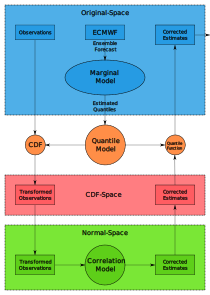
\includegraphics[width=1\linewidth]{Results/pipeline.pdf}
    \label{fig:autocorrelation:pipeline}
\end{figure}

\clearpage
\section{Model Results}
\label{autocorrelation:results}

For calculating the scores of the correlation models, Two methods was used:

As mentioned in \cref{data:ensemble} the \gls{ecmwf} forecast for a given day are available in its entirety 12 hours before the day.

For the first evaluation method the correlation models were provided with all observations up to 12 hours before the current time, corresponding to all information available at the time of the original forecasts.

In the second evaluation method the correlation model was given no observational data. In practice accomplished by forecasting a very long time horizon, $24000$ hours, and using only the last 24 hours.

An example of the \gls{sarma} forecasts compared to the feature model forecast, can be seen in \cref{fig:autocorrelation:dk1-example}, with examples for all zones in available in the appendix \cref{appendix:autocorrelation:sarma}. 

The examples are only for the \gls{sarma} models with observational data, the forecasts without observational data are nearly identical to the base feature model forecast.

\begin{figure}[htb]
    \centering
    \caption[Example SARMA Forecast]{Example of the \gls{sarma} forecast for DK1-onshore.}
    \includegraphics[width=1\linewidth]{Results/Autocorrelation/Figures/DK1-onshore example.pdf}
    \label{fig:autocorrelation:dk1-example}
\end{figure}

From the examples, the correlation models seem to better follow the trajectories of the observations. Allowing the estimates to respond when periods of deviations occurs.

\subsection{Scores}
Finally, the scores of the correlation corrected forecasts can be calculated, the scores can be seen in \cref{tab:autocorrelation:scores}

\begin{table}[htb]
\centering
\caption[Marginal Distribution Scores.]{Scores for the estimated marginal distributions. Bold scores indicated the minimum scores for the the zone and measure. Scores colored blue are within 10\% of the minimum score}
\label{tab:autocorrelation:scores}
\begin{tabular}{llrrrr}
\toprule
 &  & MAE & RMSE & CRPS & VarS \\
 & Model &  &  &  &  \\
\midrule
\multirow[r]{5}{*}{DK1-offshore} & Ensemble & {\cellcolor[HTML]{269BE3}} 127.79 & {\cellcolor[HTML]{269BE3}} 184.71 & 99.71 & {\cellcolor[HTML]{269BE3}} 30.09 \\
 & Ensemble - Raw & {\cellcolor[HTML]{269BE3}} 127.57 & {\cellcolor[HTML]{269BE3}} 182.66 & 100.78 & 34.00 \\
 & Feature & {\cellcolor[HTML]{269BE3}} 124.55 & {\cellcolor[HTML]{269BE3}} 183.81 & {\cellcolor[HTML]{269BE3}} 90.21 & 34.65 \\
 & SARMA & \bfseries \itshape {\cellcolor[HTML]{269BE3}} 118.65 & \bfseries \itshape {\cellcolor[HTML]{269BE3}} 173.51 & \bfseries \itshape {\cellcolor[HTML]{269BE3}} 85.23 & \bfseries \itshape {\cellcolor[HTML]{269BE3}} 29.56 \\
 & SARMA - no obs & {\cellcolor[HTML]{269BE3}} 124.25 & {\cellcolor[HTML]{269BE3}} 183.07 & {\cellcolor[HTML]{269BE3}} 90.18 & {\cellcolor[HTML]{269BE3}} 29.95 \\
\hline
\multirow[r]{5}{*}{DK1-onshore} & Ensemble & {\cellcolor[HTML]{269BE3}} 197.40 & {\cellcolor[HTML]{269BE3}} 269.89 & {\cellcolor[HTML]{269BE3}} 145.62 & 42.11 \\
 & Ensemble - Raw & {\cellcolor[HTML]{269BE3}} 199.37 & {\cellcolor[HTML]{269BE3}} 270.60 & {\cellcolor[HTML]{269BE3}} 145.71 & 41.97 \\
 & Feature & {\cellcolor[HTML]{269BE3}} 201.68 & {\cellcolor[HTML]{269BE3}} 282.26 & {\cellcolor[HTML]{269BE3}} 142.00 & 49.17 \\
 & SARMA & \bfseries \itshape {\cellcolor[HTML]{269BE3}} 190.80 & \bfseries \itshape {\cellcolor[HTML]{269BE3}} 267.51 & \bfseries \itshape {\cellcolor[HTML]{269BE3}} 136.05 & \bfseries \itshape {\cellcolor[HTML]{269BE3}} 35.86 \\
 & SARMA - no obs & {\cellcolor[HTML]{269BE3}} 201.68 & {\cellcolor[HTML]{269BE3}} 282.26 & {\cellcolor[HTML]{269BE3}} 142.21 & {\cellcolor[HTML]{269BE3}} 37.35 \\
\hline
\multirow[r]{5}{*}{DK2-offshore} & Ensemble & 161.87 & 246.89 & 127.12 & 35.51 \\
 & Ensemble - Raw & 156.16 & 236.59 & 127.85 & 35.92 \\
 & Feature & {\cellcolor[HTML]{269BE3}} 104.54 & {\cellcolor[HTML]{269BE3}} 167.05 & {\cellcolor[HTML]{269BE3}} 77.55 & 31.02 \\
 & SARMA & \bfseries \itshape {\cellcolor[HTML]{269BE3}} 103.05 & \bfseries \itshape {\cellcolor[HTML]{269BE3}} 164.37 & \bfseries \itshape {\cellcolor[HTML]{269BE3}} 75.94 & \bfseries \itshape {\cellcolor[HTML]{269BE3}} 27.46 \\
 & SARMA - no obs & {\cellcolor[HTML]{269BE3}} 104.54 & {\cellcolor[HTML]{269BE3}} 167.05 & {\cellcolor[HTML]{269BE3}} 77.46 & {\cellcolor[HTML]{269BE3}} 27.97 \\
\hline
\multirow[r]{5}{*}{DK2-onshore} & Ensemble & 72.40 & 100.67 & 53.75 & 15.89 \\
 & Ensemble - Raw & 76.85 & 108.45 & 59.91 & 11.84 \\
 & Feature & {\cellcolor[HTML]{269BE3}} 43.60 & {\cellcolor[HTML]{269BE3}} 59.48 & {\cellcolor[HTML]{269BE3}} 30.54 & 9.85 \\
 & SARMA & \bfseries \itshape {\cellcolor[HTML]{269BE3}} 41.17 & \bfseries \itshape {\cellcolor[HTML]{269BE3}} 55.90 & \bfseries \itshape {\cellcolor[HTML]{269BE3}} 29.34 & \bfseries \itshape {\cellcolor[HTML]{269BE3}} 7.76 \\
 & SARMA - no obs & {\cellcolor[HTML]{269BE3}} 43.60 & {\cellcolor[HTML]{269BE3}} 59.48 & {\cellcolor[HTML]{269BE3}} 30.73 & {\cellcolor[HTML]{269BE3}} 7.93 \\
\hline
\multirow[r]{5}{*}{Geometric mean score} & Ensemble & 131.12 & 187.62 & 99.80 & 29.08 \\
 & Ensemble - Raw & 132.18 & 188.71 & 102.98 & 27.91 \\
 & Feature & {\cellcolor[HTML]{269BE3}} 103.44 & {\cellcolor[HTML]{269BE3}} 150.68 & {\cellcolor[HTML]{269BE3}} 74.22 & 26.86 \\
 & SARMA & \bfseries \itshape {\cellcolor[HTML]{269BE3}} 99.00 & \bfseries \itshape {\cellcolor[HTML]{269BE3}} 143.71 & \bfseries \itshape {\cellcolor[HTML]{269BE3}} 71.30 & \bfseries \itshape {\cellcolor[HTML]{269BE3}} 21.80 \\
 & SARMA - no obs & {\cellcolor[HTML]{269BE3}} 103.38 & {\cellcolor[HTML]{269BE3}} 150.53 & {\cellcolor[HTML]{269BE3}} 74.33 & {\cellcolor[HTML]{269BE3}} 22.32 \\
\bottomrule
\end{tabular}
\end{table}


For \gls{mae}, \gls{rmse}, \gls{crps} the \gls{sarma} forecast with observational data performed better in  all zones. While the scores are better it does not beat the other models by are large margin. With the feature model scoring within 10\% in all cases.

The improvement in these scores also seem to come only from the addtional information provided by the observational data. The \gls{sarma} mode without observational data score identically to the feature model.

The improvement in \gls{vars} is however quite stark, with only the ensemble forecast in DK1-offshore being close.

The largest improvement is in DK2 onshore where the scores \gls{vars} is improved by $19.5\%$ compared to the feature model to $34\%-51\%$, compared to the ensembles.

The most notable thing is how the improvement in \gls{vars} does not seem to be contingent on additional information provided by the observational data.

Across zones the improvement in \gls{vars} compared the feature model is $19\%$ with observational data, and $17\%$ without.

This would suggest the models do capture the correlation structure of the system well.